\documentclass{article}
\usepackage[UTF8]{ctex} % 中文支持
\usepackage{amsmath}
\usepackage{amssymb}
\usepackage{geometry}
\usepackage{booktabs} % 优化表格
\usepackage{tabularx}
\usepackage{graphicx}
\usepackage{float}


\geometry{a4paper, margin=1in}

\title{实验1：谐振 RLC 串联电路的频率特性\\ \large 实验报告}
\author{TCY From Dushi College}
\date{2026年4月1日}


\begin{document}

\maketitle

\tableofcontents


\newpage


\section{实验目的（预习内容）}
\begin{enumerate}
    \item 测量 R、L、C 串联电路电流响应的幅频特性。
    \item 研究串联谐振现象及其特点。
    \item 研究元件参数（如电阻 $R$、电容 $C$）对电路频率特性的影响。
    \item 熟悉函数信号发生器、数字存储示波器、万用表等仪器的使用方法。
\end{enumerate}

\section{实验仪器与设备（预习内容）}
\begin{itemize}
    \item 函数信号发生器、数字存储示波器、万用表。
    \item 实验箱（含电阻、电容、电感）、实验导线。
    \item 电感参数：$L = 100\text{mH}$，内阻 $r = 49\Omega$。
\end{itemize}

\section{实验原理与计算（预习内容）}
\subsection{谐振频率理论值}
根据 RLC 串联电路公式，谐振频率 $f_0$ 为：
$$f_0 = \frac{1}{2\pi\sqrt{LC}}$$
若 $L = 100\text{mH}$，$C = 1\mu\text{F}$，则：
$$f_0 = \frac{1}{2\pi\sqrt{0.1 \times 10^{-6}}} \approx 503.3\text{ Hz}$$

\subsection{实验要点}
\begin{itemize}
    \item \textbf{谐振判断}：通过示波器 X-Y 模式观察李萨如图形，当总电压 $u$ 与电阻电压 $u_R$（代表电流 $I$）同相时，电路发生谐振。
    \item \textbf{幅频特性测量}：保持输入电压 $U$ 恒定在 $2\text{V}$，在 $f_0$ 附近加密取点测量 $I$。
\end{itemize}


\newpage
\section{数据记录表格}

\subsection{内容一：$R=10\Omega, C=1\mu\text{F}$ 的幅频特性测量}
预期 $f_0 \approx 503\text{Hz}$。


\begin{table}[H]
\centering
\begin{tabular}{|l|c|c|c|c|c|c|}
\hline
配置 & 实测 $f_0$ (Hz) & $U$ (V) & $U_C$ (V) & $U_L$ (V) & $U_{C-L}$ (V) & $U_{R}$ (V) \\ \hline
$R=10\Omega, C=1\mu\text{F}$ & 474.0 & 2.0 & 7.77 & 7.89 & 1.72 & 0.252 \\ \hline
\end{tabular}
\end{table}

% 设置行高，方便手写
\renewcommand{\arraystretch}{1.5} 

\begin{table}[h!]
\centering
\small
\begin{tabular}{|m{2.5cm}|*{9}{>{\centering\arraybackslash}m{1.2cm}|}}
\hline
\multicolumn{10}{|l|}{\textbf{第一组：低频稀疏区及过渡区}} \\ \hline
偏移量 & $-50$ & $- 50$ & $- 20$ & $- 20$ & $- 10$ & $- 10$ & $-10$ & $- 10$ & $- 5$ \\ \hline
频率 $f$ (Hz) & 269 & 319 & 369 & 389 & 409 & 419 & 429 & 439 & 449 \\ \hline
电压 $U_R$ (mV) & 48.75 & 70.52 & 107.77 & 131.74 & 162.13 & 180.52 & 200.40 & 219.23 & 236.02 \\ \hline
电流 $I$ (mA) & 4.875 & 7.052 & 10.777 & 13.174 & 16.213 & 18.052 & 20.040 & 21.923 & 23.602 \\ \hline
\end{tabular}

\vspace{0.5cm}

\begin{tabular}{|m{2.5cm}|*{9}{>{\centering\arraybackslash}m{1.2cm}|}}
\hline
\multicolumn{10}{|l|}{\textbf{第二组：谐振核心密集区 ($f_0$ 附近)}} \\ \hline
偏移量 & $- 5$ & $- 5$ & $-5$ & $- 5$ & \boldmath{$f_0$} & $+ 5$ & $+5$ & $+ 5$ & $+ 5$ \\ \hline
频率 $f$ (Hz) & 454 & 459 & 464 & 469 & 474 & 479 & 484 & 489 & 494 \\ \hline
电压 $U_R$ (mV) & 244.55 & 249.72 & 253.33 & 256.55 & 257.20 & 256.99 & 255.00 & 251.11 & 246.82 \\ \hline
电流 $I$ (mA) & 24.455 & 24.972 & 25.333 & 25.655 & 25.720 & 25.699 & 25.500 & 25.111 & 24.682 \\ \hline
\end{tabular}

\vspace{0.5cm}

\begin{tabular}{|m{2.5cm}|*{9}{>{\centering\arraybackslash}m{1.2cm}|}}
\hline
\multicolumn{10}{|l|}{\textbf{第三组：高频过渡区及稀疏区}} \\ \hline
偏移量 & $+ 5$ & $+ 10$ & $+ 10$ & $+10$ & $+10$ & $+ 20$ & $+20$ & $+50$ & $+ 50$ \\ \hline
频率 $f$ (Hz) & 499 & 509 & 519 & 529 & 539 & 559 & 579 & 629 & 679 \\ \hline
电压 $U_R$ (mV) & 242.14 & 230.15 & 217.38 & 204.89 & 192.57 & 169.46 & 150.89 & 115.47 & 92.90 \\ \hline
电流 $I$ (mA) & 24.214 & 23.015 & 21.738 & 20.489 & 19.257 & 16.946 & 15.089 & 11.547 & 9.290 \\ \hline
\end{tabular}
\caption{幅频特性数据记录表（共 27 个点，需边测边调 $U$ 保持在 2V 左右）}
\end{table}

% 恢复默认行高
\renewcommand{\arraystretch}{1}

\newpage

\subsection{内容二：$R=30\Omega, C=1\mu\text{F}$ 情况}


\begin{table}[H]
\centering
\begin{tabular}{|l|c|c|c|c|c|c|}
\hline
配置 & 实测 $f_0$ (Hz) & $U$ (V) & $U_C$ (V) & $U_L$ (V) & $U_{C-L}$ (V) & $U_{R}$ (V) \\ \hline
$R=30\Omega, C=1\mu\text{F}$  & 477.0 & 2.0 & 6.30  & 6.37&1.381 &0.609 \\ \hline
\end{tabular}
\end{table}

% 设置行高，方便手写
\renewcommand{\arraystretch}{1.5} 

\begin{table}[H]
\centering
\small
\begin{tabular}{|m{2.5cm}|*{9}{>{\centering\arraybackslash}m{1.2cm}|}}
\hline
\multicolumn{10}{|l|}{\textbf{第一组：低频稀疏区及过渡区}} \\ \hline
偏移量 & $-50$ & $- 50$ & $- 20$ & $- 20$ & $- 10$ & $- 10$ & $-10$ & $- 10$ & $- 5$ \\ \hline
频率 $f$ (Hz) & 272.0 & 322.0 & 372.0 & 392.0 & 412.0 & 422.0 & 432.0 & 442.0 & 452.0 \\ \hline
电压 $U_R$ (mV) & 147.02 & 209.93 & 310.82 & 370.23 & 441.18 & 478.96 & 517.30 & 550.82 & 582.80 \\ \hline
电流 $I$ (mA) & 4.90 & 7.00 & 10.36 & 12.34 & 14.71 & 15.97 & 17.24 & 18.36 & 19.43 \\ \hline
\end{tabular}

\vspace{0.5cm}

\begin{tabular}{|m{2.5cm}|*{9}{>{\centering\arraybackslash}m{1.2cm}|}}
\hline
\multicolumn{10}{|l|}{\textbf{第二组：谐振核心密集区 ($f_0$ 附近)}} \\ \hline
偏移量 & $- 5$ & $- 5$ & $-5$ & $- 5$ & \boldmath{$f_0$} & $+ 5$ & $+5$ & $+ 5$ & $+ 5$ \\ \hline
频率 $f$ (Hz) & 457.0 & 462.0 & 467.0 & 472.0 & 477.0 & 482.0 & 487.0 & 492.0 & 497.0 \\ \hline
电压 $U_R$ (mV) & 594.80 & 602.56 & 609.00 & 613.02 & 614.90 & 616.35 & 611.95 & 608.53 & 602.21 \\ \hline
电流 $I$ (mA) & 19.83 & 20.09 & 20.30 & 20.43 & 20.50 & 20.55 & 20.40 & 20.28 & 20.07 \\ \hline
\end{tabular}

\vspace{0.5cm}

\begin{tabular}{|m{2.5cm}|*{9}{>{\centering\arraybackslash}m{1.2cm}|}}
\hline
\multicolumn{10}{|l|}{\textbf{第三组：高频过渡区及稀疏区}} \\ \hline
偏移量 & $+ 5$ & $+ 10$ & $+ 10$ & $+10$ & $+10$ & $+ 20$ & $+20$ & $+50$ & $+ 50$ \\ \hline
频率 $f$ (Hz) & 502.0 & 512.0 & 522.0 & 532.0 & 542.0 & 562.0 & 582.0 & 632.0 & 682.0 \\ \hline
电压 $U_R$ (mV) & 592.23 & 573.84 & 549.18 & 524.11 & 500.43 & 451.90 & 408.54 & 322.81 & 264.18 \\ \hline
电流 $I$ (mA) & 19.74 & 19.13 & 18.31 & 17.47 & 16.68 & 15.06 & 13.62 & 10.76 & 8.81 \\ \hline
\end{tabular}
\caption{幅频特性数据记录表（$R=30\,\Omega$，$I = U_R/30$）}
\end{table}
% 恢复默认行高
\renewcommand{\arraystretch}{1}

\subsection{内容3：$R=10\Omega, C=0.5\mu\text{F}$ 情况}
预期 $f_0 \approx 712\text{Hz}$。
\begin{table}[H]
\centering
\begin{tabular}{|l|c|c|c|c|c|c|}
\hline
配置 & 实测 $f_0$ (Hz) & $U$ (V) & $U_C$ (V) & $U_L$ (V) & $I_0$ (mA)  \\ \hline
$R=10\Omega, C=0.5\mu\text{F}$ & 704.4 & 2.0 &13.25 & 13.34& 0.27\\ \hline
\end{tabular}
\end{table}

\newpage

\section{实验结果分析}
\subsection{频幅特性曲线$I(f)$}
\begin{figure}[H]
    \centering
    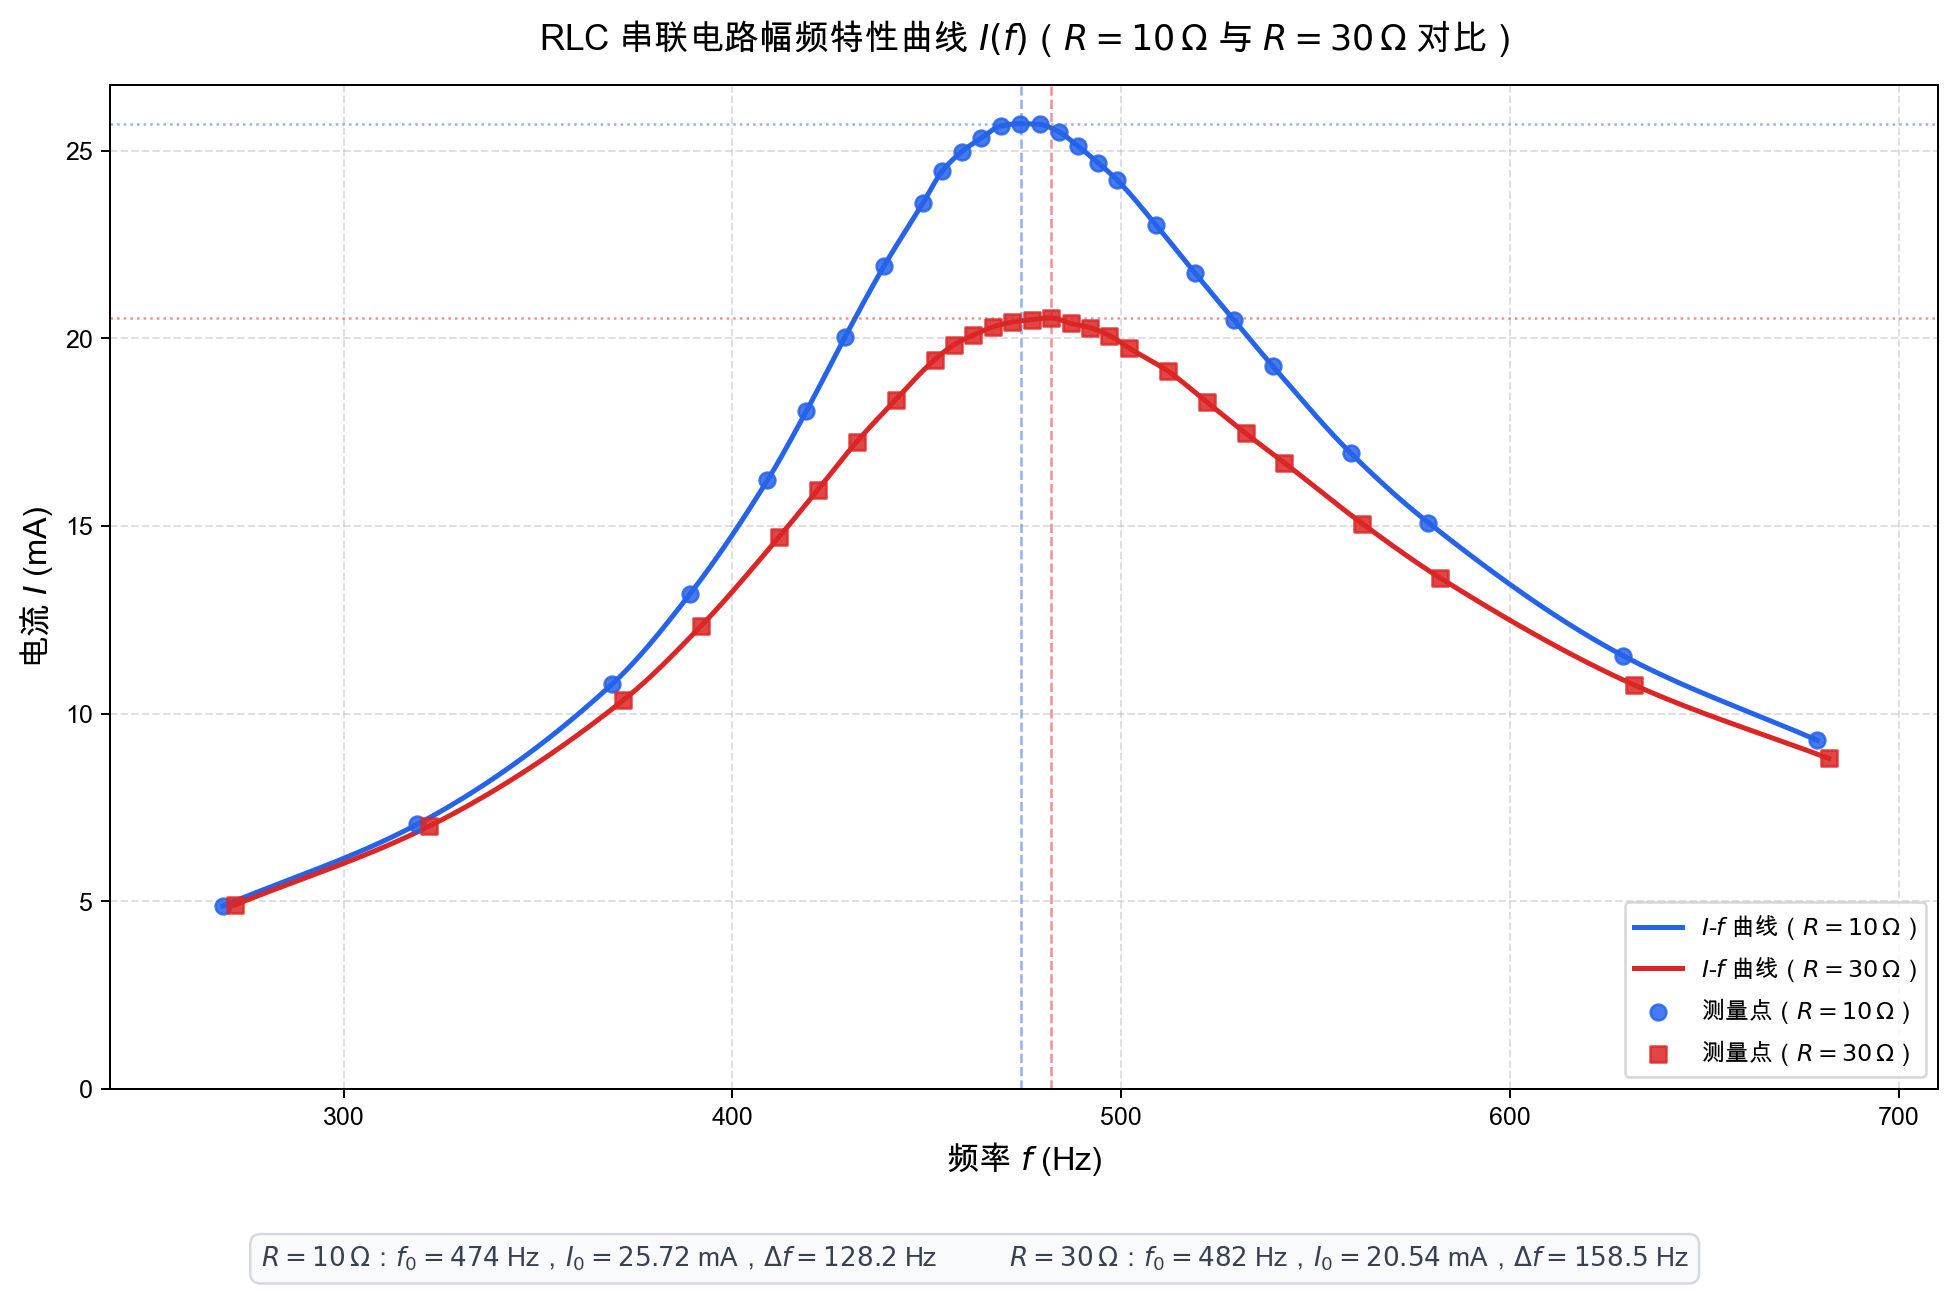
\includegraphics[width=1\linewidth]{RLC_combined_I_f_curve.png}
    \caption{$I(f)曲线$}
    \label{fig:placeholder}
\end{figure}

\subsection{$I(f)$曲线的分析}
通过对不同电阻下的 RLC 串联电路幅频特性曲线进行对比，可以总结出以下异同点：

\begin{itemize}
    \item \textbf{谐振频率的稳定性（同）}：实验测得 $R=10\,\Omega$ 与 $R=30\,\Omega$ 时的谐振频率 $f_0$ 分别为 $474\,\text{Hz}$ 和 $482\,\text{Hz}$。两者基本一致且接近理论值（约 $503.3\,\text{Hz}$），验证了谐振频率主要由电路中的感容元件 $L$ 和 $C$ 决定，受电阻 $R$ 影响较小。
    \item \textbf{电阻对幅值与带宽的影响（异）}：
    \begin{enumerate}
        \item \textbf{幅值}：电阻 $R$ 越小，谐振时的总阻抗越小，电流峰值越高。图中蓝色曲线 ($10\,\Omega$) 的峰值电流 ($25.72\,\text{mA}$) 明显高于红色曲线 ($30\,\Omega$) 的 $20.54\,\text{mA}$。
        \item \textbf{带宽与选择性}：$R=10\,\Omega$ 时的带宽 $\Delta f = 128.2\,\text{Hz}$，小于 $R=30\,\Omega$ 时的 $158.5\,\text{Hz}$。这说明电阻越小，电路的品质因数 $Q$ 越高，曲线越尖锐，电路的选择性越好。
    \end{enumerate}
\end{itemize}

\subsection{利用实测电容值计算真实电感}
根据串联谐振公式 $f_0 = \frac{1}{2\pi\sqrt{LC}}$，可推导出电感的计算表达式为：
\begin{equation}
L = \frac{1}{(2\pi f_0)^2 C}
\end{equation}
注：我在实验中遗漏了对电容$C$的值的测量，因此在此节中使用$C$的标定值进行计算。
代入第一组实验数据：实测谐振频率 $f_0 = 474.0\text{ Hz}$，实测电容 $C = 1.0 \times 10^{-6}\text{ F}$，计算得：
\begin{equation}
L = \frac{1}{(2\pi \times 474.0)^2 \times 1.0 \times 10^{-6}} \approx 0.1128\text{ H} = 112.8\text{ mH}
\end{equation}
\subsection{总结谐振特点，分析$U_{C-L}$, 估算电感谐振时的电阻}
\subsubsection{总结谐振特点}
R、L、C 串联电路发生谐振时具有以下主要特点：
\begin{enumerate}
    \item \textbf{阻抗最小}：电路的总阻抗呈现纯电阻性，即 $Z = R_{total}$，阻抗达到最小值。
    \item \textbf{电流最大}：在激励电压 $U$ 不变的情况下，电路中的电流达到最大值 $I_0 = U / R_{total}$。
    \item \textbf{相位同相}：输入电压 $u$ 与电路电流 $i$ 同相位。
    \item \textbf{电压关系}：电感电压 $\dot{U}_L$ 与电容电压 $\dot{U}_C$ 大小相等、相位相反，相互抵消。
\end{enumerate}

\subsubsection{分析 $U_{C-L}$}
在理想情况下（即电感无内阻），谐振时电感和电容的电抗完全抵消，其相量和应为 0。但在实际电路中，必须考虑电感的直流内阻 $r$（实验给定 $r=49\,\Omega$）。根据相量模型，谐振时 $\dot{U}_L + \dot{U}_C = \dot{I}_0(r + jX_L) + \dot{I}_0(-jX_C)$。由于 $X_L = X_C$，理论上 $U_{C-L}$ 的有效值应满足：
\begin{equation}
U_{C-L} = I_0 \cdot r = \frac{U_R}{R} \cdot r
\end{equation}

根据实验总结表数据进行计算：
\begin{itemize}
    \item \textbf{当 $R=10\,\Omega$ 时}：电流 $I_0 = 0.252 / 10 = 25.2\text{ mA}$。理论预期 $U_{C-L} \approx 25.2\text{ mA} \times 49\,\Omega \approx 1.235\text{ V}$。实测值为 $1.72\text{ V}$。
    \item \textbf{当 $R=30\,\Omega$ 时}：电流 $I_0 = 0.609 / 30 = 20.3\text{ mA}$。理论预期 $U_{C-L} \approx 20.3\text{ mA} \times 49\,\Omega \approx 0.995\text{ V}$。实测值为 $1.381\text{ V}$。
\end{itemize}
观察发现，两组实验的实测值均明显高于基于直流电阻计算的理论值。这说明在谐振频率下，电感线圈的等效电阻（交流电阻）受趋肤效应及磁芯损耗影响，要大于其直流电阻 $r$。

\subsubsection{估算电感谐振时的电阻}
谐振时电路呈纯电阻性，总等效电阻为 $R_{total} = U / I_0$。电感的交流等效电阻 $r_{ac}$ 可通过 $r_{ac} = R_{total} - R$ 估算。

\begin{enumerate}
    \item \textbf{当 $R=10\,\Omega$ 时}：
    $$R_{total, 1} = \frac{2.0\text{ V}}{25.2\text{ mA}} \approx 79.37\,\Omega \implies r_{ac, 1} = 79.37 - 10 = 69.37\,\Omega$$
    \item \textbf{当 $R=30\,\Omega$ 时}：
    $$R_{total, 2} = \frac{2.0\text{ V}}{20.3\text{ mA}} \approx 98.52\,\Omega \implies r_{ac, 2} = 98.52 - 30 = 68.52\,\Omega$$
\end{enumerate}

\textbf{结论}：两组实验估算出的电感交流电阻 $r_{ac}$（约为 $69\,\Omega$）基本一致，且均显著大于直流电阻 $r=49\,\Omega$。这验证了在交流电路中，电感的损耗不仅包含直流线圈电阻损耗，还包括高频下的交流损耗，因此\textbf{电感谐振时的电阻与直流电阻是不相等的}。

\subsection{元件参数对电路频率特性的影响}
从实验数据和理论公式 $f_0 = \frac{1}{2\pi\sqrt{LC}}$，$Q = \frac{1}{R}\sqrt{\frac{L}{C}}$，$\Delta f = \frac{R}{2\pi L}$ 进行分析：
\begin{itemize}
    \item \textbf{对谐振频率 $f_0$ 的影响}：$f_0$ 主要由 $L$ 和 $C$ 决定。实验对比内容 1 和内容 3 可知，当 $C$ 减小（$1\mu\text{F} \to 0.5\mu\text{F}$）时，$f_0$ 显著升高；而内容 1 与内容 2 对比显示，改变电阻 $R$ 对 $f_0$ 几乎没有影响。
    \item \textbf{对品质因数 $Q$ 的影响}：$Q$ 与 $R$ 成反比，与 $\sqrt{L/C}$ 成正比。实验中 $R=10\Omega$ 的电流曲线比 $R=30\Omega$ 更尖锐，说明电阻越小，$Q$ 值越高，电路的电压放大倍数（$U_C/U$ 或 $U_L/U$）也越大。
    \item \textbf{对通频带宽度 $\Delta f$ 的影响}：$\Delta f$ 与 $R$ 成正比。电阻 $R$ 越大，幅频特性曲线越平坦，通频带越宽，电路的选择性越差；反之，电阻越小，曲线越尖锐，选择性越好。
\end{itemize}
\section{体会}
\begin{enumerate}
    \item  实验过程中每一次调整信号发生器的频率，都要调整电压值（维持为2.0V）。
    \item  考虑电感元件的内阻，并且考虑交流电阻和直流电阻的差异
    \item  为了平衡精确度和工作量，记录数据时，在平缓处可以适量减少数据的记录，在变化剧烈处应增加记录点的数量。
\end{enumerate}

\section{预习报告、原始数据与助教签名}
\begin{figure}[htbp]
    \centering
    \begin{minipage}[t]{0.48\textwidth}
        \centering
        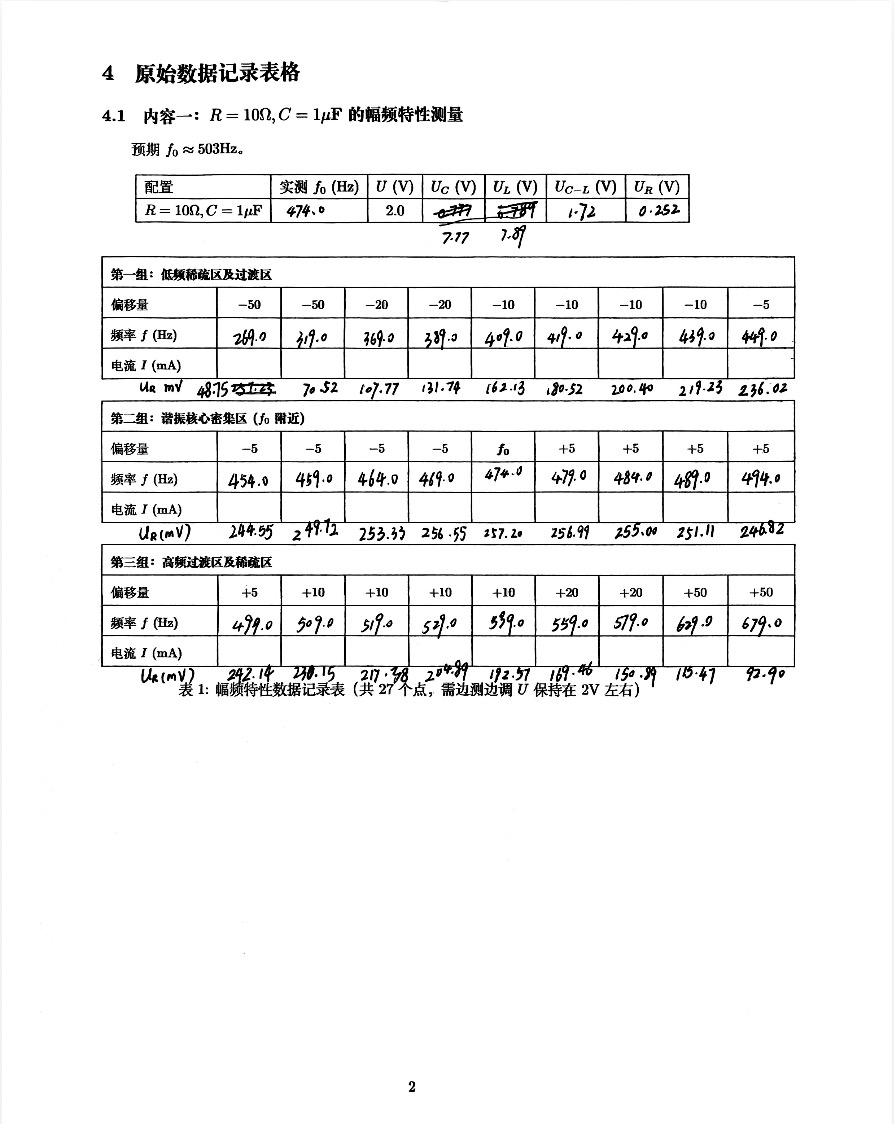
\includegraphics[width=\textwidth]{原始数据1.jpg}
        \caption{原始数据1}
    \end{minipage}
    \hfill
    \begin{minipage}[t]{0.48\textwidth}
        \centering
        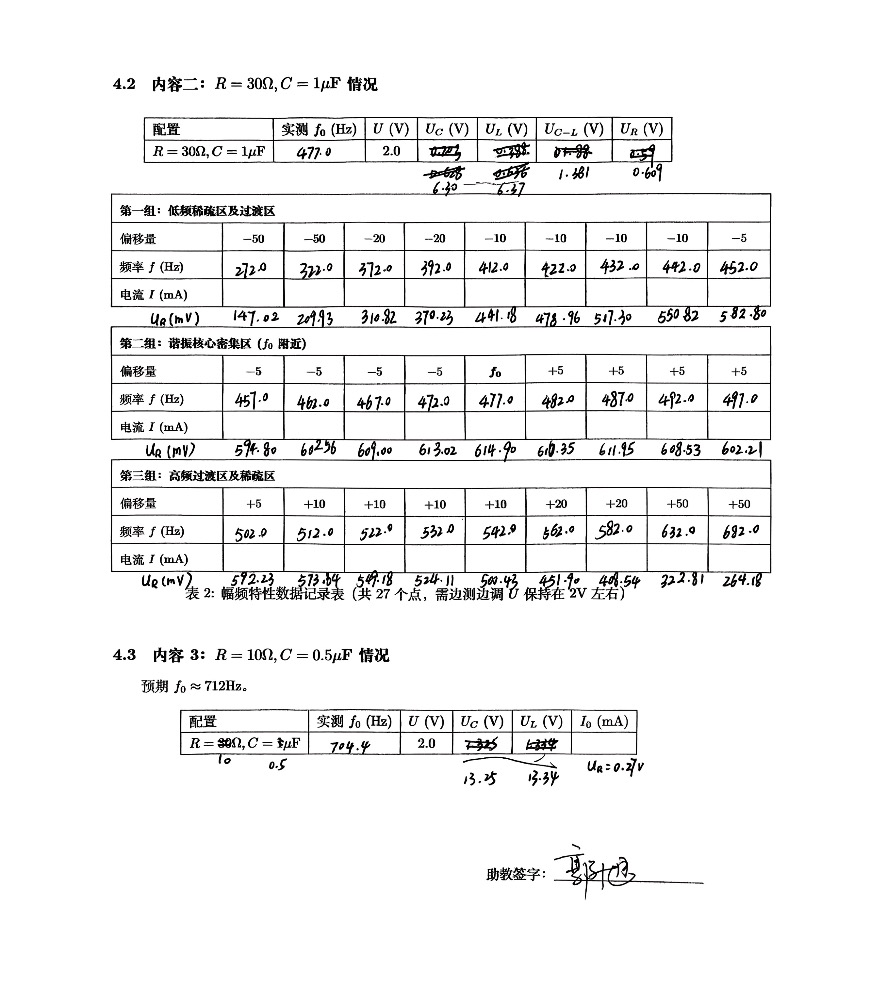
\includegraphics[width=\textwidth]{原始数据2.jpg}
        \caption{原始数据2}
    \end{minipage}
\end{figure}

\begin{figure}
    \centering
    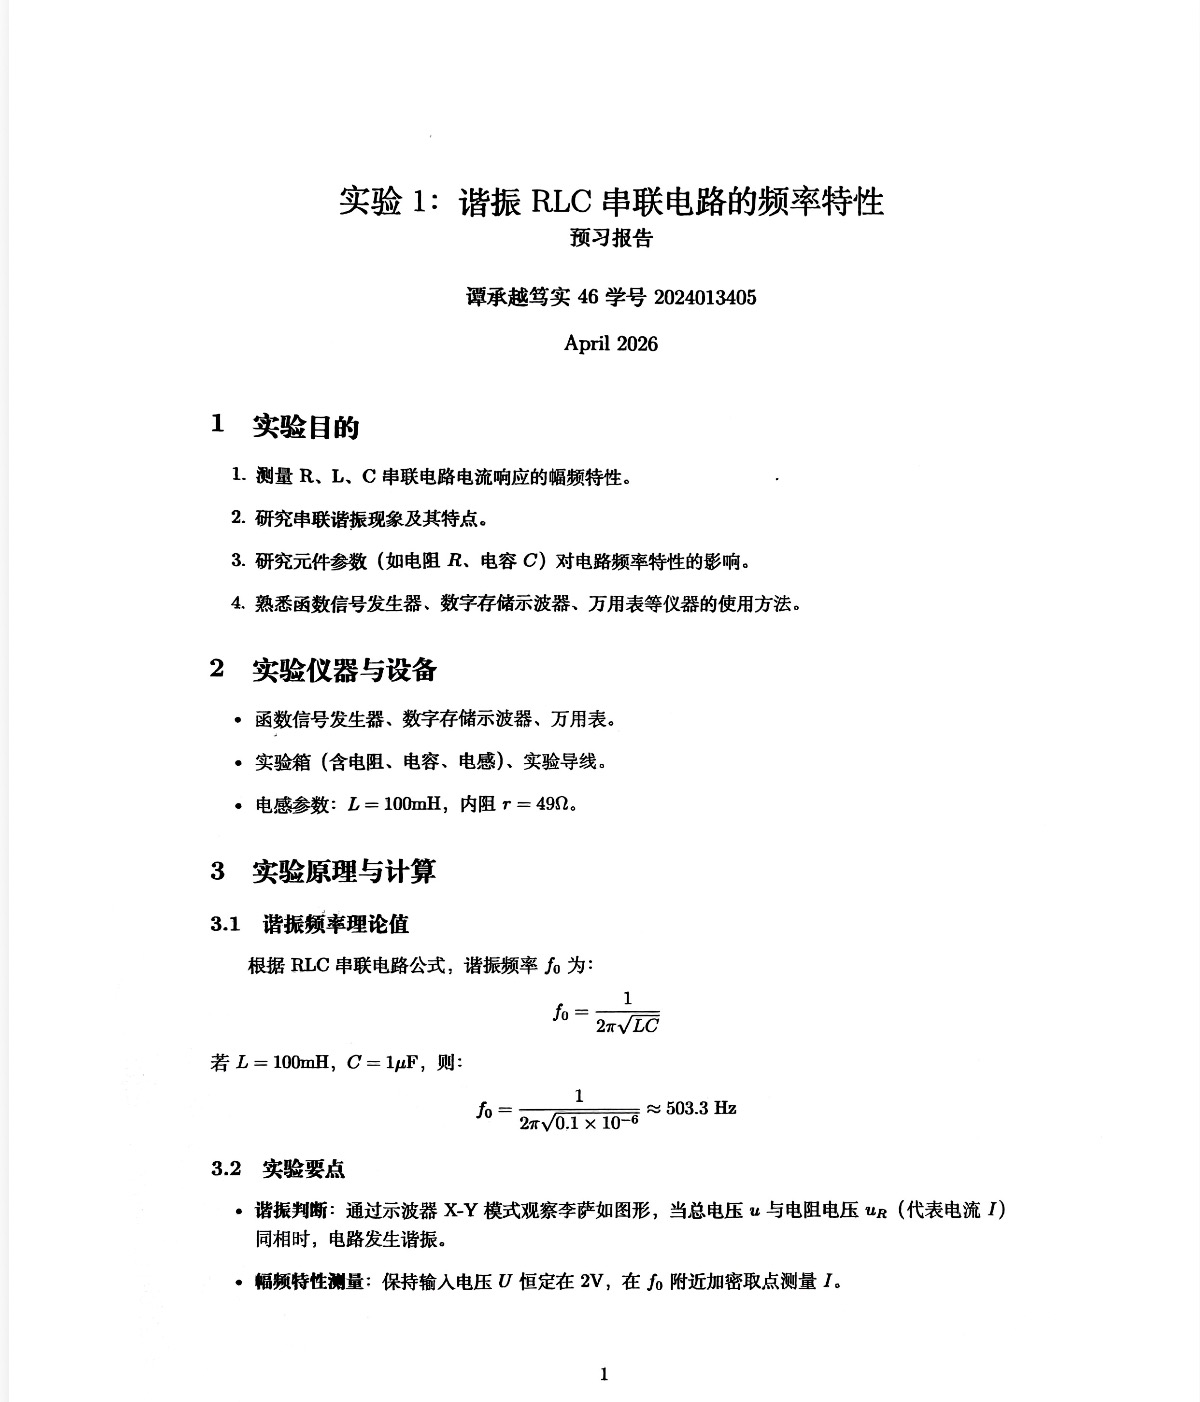
\includegraphics[width=1\linewidth]{img 2026-04-01 19.37.53.jpg}
    \caption{预习报告}
    \label{fig:placeholder}
\end{figure}


\end{document}
